\documentclass{article}
\usepackage{graphicx} % Required for inserting images
\usepackage[margin=2cm, top=3cm]{geometry} % margine superiore ridotto a 1 cm
\usepackage{listings}
\usepackage{subcaption}  % Pacchetto per sottodidascalie
\usepackage{float}       % Pacchetto per posizionamento rigido delle figure

\begin{document}

\section{La contabilità Direzionale}
\subsection{Cos'è la contabilità direzionale?}
La \textbf{contabilità direzionale} (management accounting) è il processo che fornisce gran parte delle informazioni utilizzate dal management per pianificare, porre in atto e controllare le attività di una organizzazione. La maggior parte dei principi applicati nello sviluppo della contabilità direzionale è indipendente dal tipo di organizzazione. Il management accounting fornisce alcune delle informazioni che aiutano i dirigenti a svolgere i loro compiti. Le informazioni che utilizzano i manager sono di natura diversa: contabili e non contabili, quantitative e non quantitative. Il management è interessato a disporre di sintesi riferite a porzioni dell'impresa, non a conoscere i singoli dettagli. In generale, le informazioni di contabilità direzionale sono pertanto informazioni riepilogative ottenute assemblando dati elementari operativi.
\subsection{Le persone che si occupano di contabilità direzionale}
I membri di un'organizzazione responsabili della progettazion e della gestione del sistema di contabilità direzionale sono gli addetti alla contabilità direzionale. In molte imprese la persona di più alto livello gerarchico tra coloro che si occupano della contabilità direzionale è chiamata \textbf{controller}. Nelle organizzazioni di piccole dimensioni il controller risponde direttmente al direttore generale. Molti direttori amministrativi sono anche controller. Nelle imprese di maggiori dimensioni le responsabilità del controller sono principalmente rivolte verso l'interno dell'organizzazione e si esplicano nel fornire informazioni utili al management. Per contro, compiti che coinvolgono maggiormente relazioni con l'esterno, come la gestione delle liquidità e di altre attività di natura monetaria, l'ottenimento di finanziamenti a titolo di credito e a titolo di rischio o l'acquisto delle polizze assicurative, sono generalmente di responsabilità di un dirigente amministrativo detto anche \textbf{responsabile della tesoreria}, anch'egli alle dipendenze del direttore amministrativo.
\subsection{Le differenze tra contabilità direzionale e contabilià generale}
La contabilità generale differisce in molti aspetti dalla contabilità direzionale: 
\begin{figure}[H] % Usa 'H' per forzare la posizione qui
    \centering % Centra l'immagine
    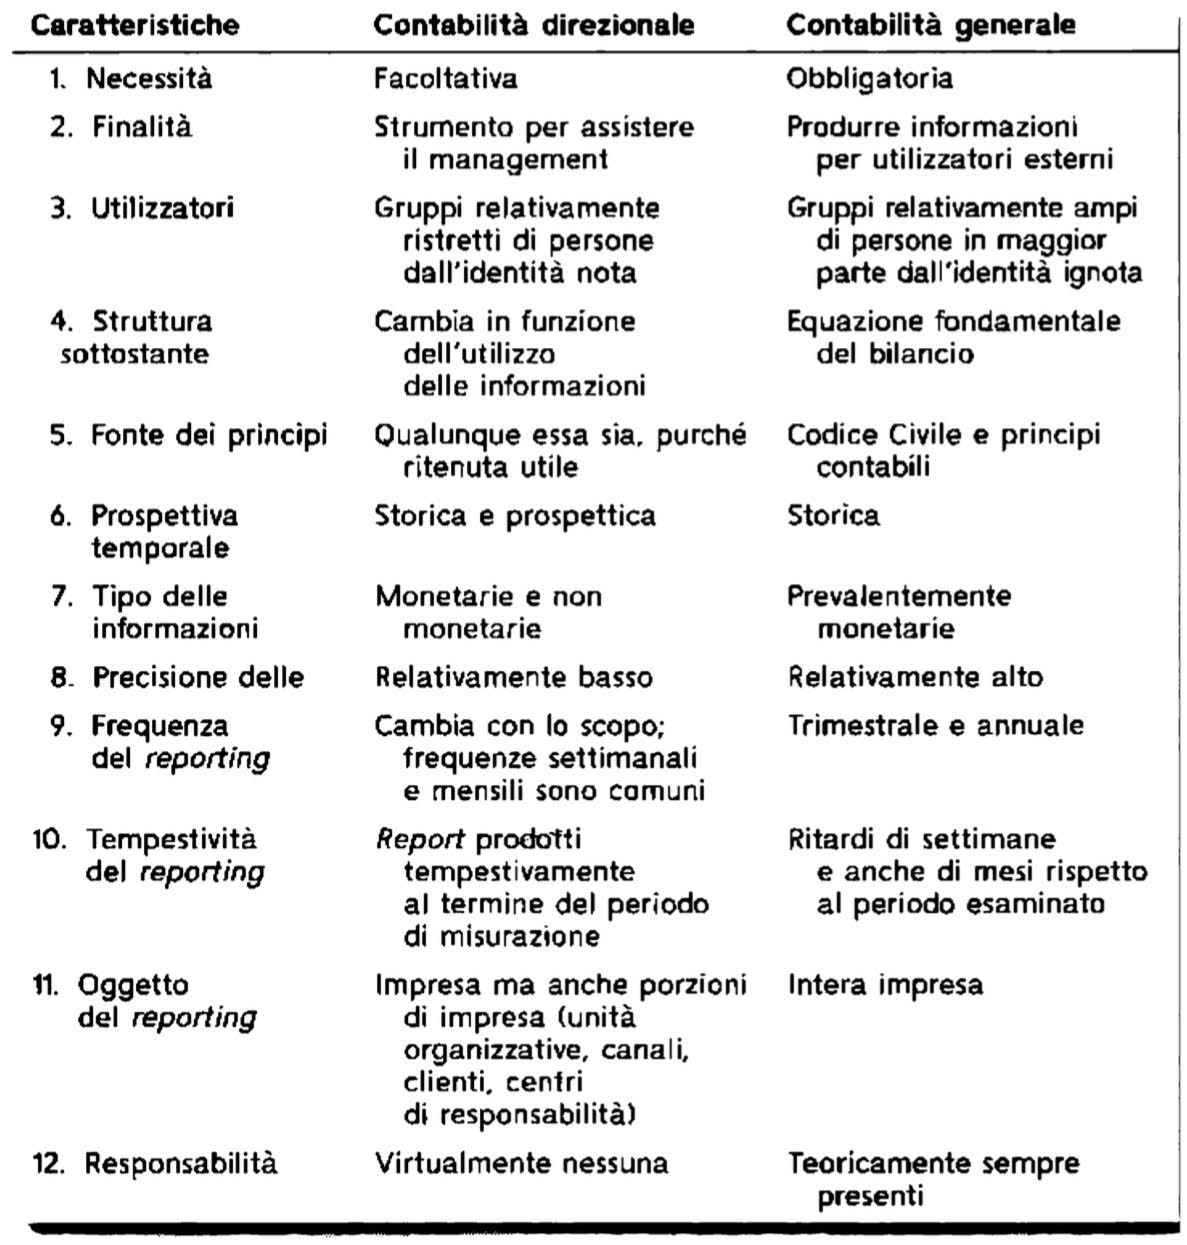
\includegraphics[width=8cm, height=9cm]{unnamed (5).jpg} % Percorso dell'immagine
    \caption{Differenze tra contabilità direzionale e contabilità generale} % Didascalia per l'immagine
    \label{fig:immagine} % Etichetta per riferimento
\end{figure}
\noindent
\paragraph{Necessità di disporre del sistema:} La contabilità generale deve obbligatoriamente esistere. Un impegno adeguato deve essere indirizzato alla raccolta dei dati in modo che questi abbiano un contenuto, una forma e un grado di accurtezza in grado di soddisfare i requisiti stabiliti dal Codice Civile e di principi contabili. La contabilità direzionale, al contrario, è discrezionale: non esistono enti o istituzioni esterne che specifichino che cosa debba essere fatto o se qualcosa debba essere fatto.
\paragraph{Lo scopo}: Lo scopo della contabilità generale è produrre informazioni per tutti i soggetti esterni interessati alla prestazione economico finanziaria dell'azienda, denominati \textbf{portatori di interessi} (stakeholder). Le informazioni della contabilità direzionale sono invece un mezzo per raggiungere uno scopo: la pianificazione, l'attuazione e il controllo delle attività del management.
\paragraph{Gli utilizzatori}: Gli utenti delle informazioni prodotte dalla contabilità generale sono spesso costituiti da attori o persone esterni all'azienda non bene identificati, oltre che dallo stesso management.
\paragraph{}
\end{document}
ànò